%Praesentationsmodus
\documentclass[t,aspectratio=169,divpsnames]{beamer}
%Die Beameroption aspectratio legt das verwendete Seitenverhaeltnis fest
%aspectratio=169	16:9 Seitenverhaeltnis
%aspectratio=1610	16:10 Seitenverhaeltnis
%aspectratio=43		4:3 Seitenverhaeltnis
%Die Beameroption envcountsect nummeriert Umgebungen wie theorem pro section durch.
%Die Beameroption divpsnames wird an das xcolor Paket durchgereicht.

%Handout-Generierung mit Foliennotizen (statt obiger Zeile für den Präsentationsmodus verwenden)
%\documentclass[t,handout,aspectratio=169]{beamer}
%\setbeameroption{show notes}

\usepackage[utf8]{inputenc}

% Deutsch
\usepackage[ngerman]{babel} 
\usepackage{bibgerm}

% Englisch
%\usepackage[english]{babel}

\usepackage{listings}
\lstset
{
	basicstyle=\tiny\linespread{0.9}\ttfamily, 	% print whole listing small
	keywordstyle=\color{blue}\bfseries,
								% underlined bold black keywords
	identifierstyle=, 			% nothing happens
	commentstyle=\color{green}, 	% white comments	
	showstringspaces=false, 	% no special string spaces
	tabsize=3,
	showtabs=false,
	rulesepcolor=\color{blue},
	linewidth=146mm
}

\lstdefinelanguage{custom}
{
morekeywords= { abstract, event, new, struct,
                as, explicit, null, switch,
                base, extern, object, this,
                bool, false, operator, throw,
                break, finally, out, true,
                byte, fixed, override, try,
                case, float, params, typeof,
                catch, for, private, uint,
                char, foreach, protected, ulong,
                checked, goto, public, unchecked,
                class, if, readonly, unsafe,
                const, implicit, ref, ushort,
                continue, in, return, using,
                decimal, int, sbyte, virtual,
                default, interface, sealed, volatile,
                delegate, internal, short, void,
                do, is, sizeof, while,
                double, lock, stackalloc,
                else, long, static,
                enum, namespace, string, var, await, async, get, set },
morestring = *[d]{"},
stringstyle=\ttfamily\color{red}
}  

\mode<presentation>
{
\usetheme{HochschuleTrier}
\setbeamercovered{transparent}
}

%\usepackage{mathptmx}
%\usepackage[scaled=0.9]{helvet}
\usepackage{helvet}
\usepackage{courier}
%\usepackage{ae}

\usepackage{hyperref}
\usepackage{tikz}
\usepackage{amsmath}
\usepackage{amsfonts}

\logo{
\includegraphics[height=7.5mm]{HochschuleLogo}}

\usetikzlibrary{calc,positioning}

\usefonttheme[onlymath]{serif}


% Stil des Literaturverzeichnisses
%\bibliographystyle{geralpha}
%\bibliographystyle{alpha}
\bibliographystyle{abstract}

%Bitte ausfuellen:
\title[Entwurf und Implementierung einer DSL zur Spezifikation von Konversationsrouting]{Entwurf und Implementierung einer grafischen, domänenspezifischen Sprache zur Spezifizierung des Konversationsrouting in Contactcentern}
%\subtitle{Titelzusatz}
\author{David Wichter}
\institute{Hochschule Trier}
\date{28.02.2018}
\subject{Thema für PDF-Metadaten (optional)}

%Inhaltsverzeichnisses bis auf subsubsection-Ebene:
%\setcounter{tocdepth}{3}

%Aktivieren, um am Anfang jeder Section ein Inhaltsverzeichnis zur Section anzuzeigen
%\AtBeginSection[]
%{
%\begin{frame}<beamer>
%\frametitle{Agenda}
%\tableofcontents[currentsection,hideothersubsections,sectionstyle=show/hide,subsubsectionstyle=show/show]
%\end{frame}
%}

%Aktivieren, um alles Schritt-fuer-Schritt einzublenden
%\beamerdefaultoverlayspecification{<+->}
\setbeamercovered{invisible}

\defbeamertemplate{description item}{align left}{\insertdescriptionitem\hfill}

\begin{document}

\begin{frame}
\titlepage
\end{frame}

%\begin{frame}
%	\frametitle{Agenda}
%	\tableofcontents
%	%\tableofcontents[hideallsubsections] % Subsections ausblenden
%	%\tableofcontents[pausesections] %Sections Schritt-fuer-Schritt einblenden
%\end{frame}

\begin{frame}{Einführung}{Wer?}
	\only<1->
	{
		\begin{figure}
			\includegraphics[scale=0.08]{img/ilogixx_logo.png}
		\end{figure}
	}
	\only<2->
	{
		\begin{figure}
			\includegraphics[scale=0.65]{img/mycontactcenter_logo.jpeg}
		\end{figure}
	}
\end{frame}

\begin{frame}{Einführung}{Was?}
	\begin{columns}[T]
		\setbeamertemplate{description item}[align left]
		\begin{column}{0.55\textwidth}
			\only<2->
			{
				\begin{description}[MyCC-Server]
					\item<2->[Konversation] Informationsaustausch über beliebigen Kanal
					\item<3->[ACD] Automatic Conversation Distribution	
					\item<4->[Agent] Contactcenter-Teilnehmer
					\item<5->[MyCC-Server] Zentrale Verwaltungskomponente		
					\item<6->[IP-PBX] IP-Private Branch Exchange
					\item<7->[SIP] Session Initiation Protocol
				\end{description}
			}
		\end{column}
		\begin{column}{0.45\textwidth}
				\only<1-7>
				{
					\vspace{0.5cm}
        			\includegraphics[scale=0.4]{img/MyCC_logo.jpg}
				}        		
        		\only<8>
				{
					\vspace{0.5cm}
					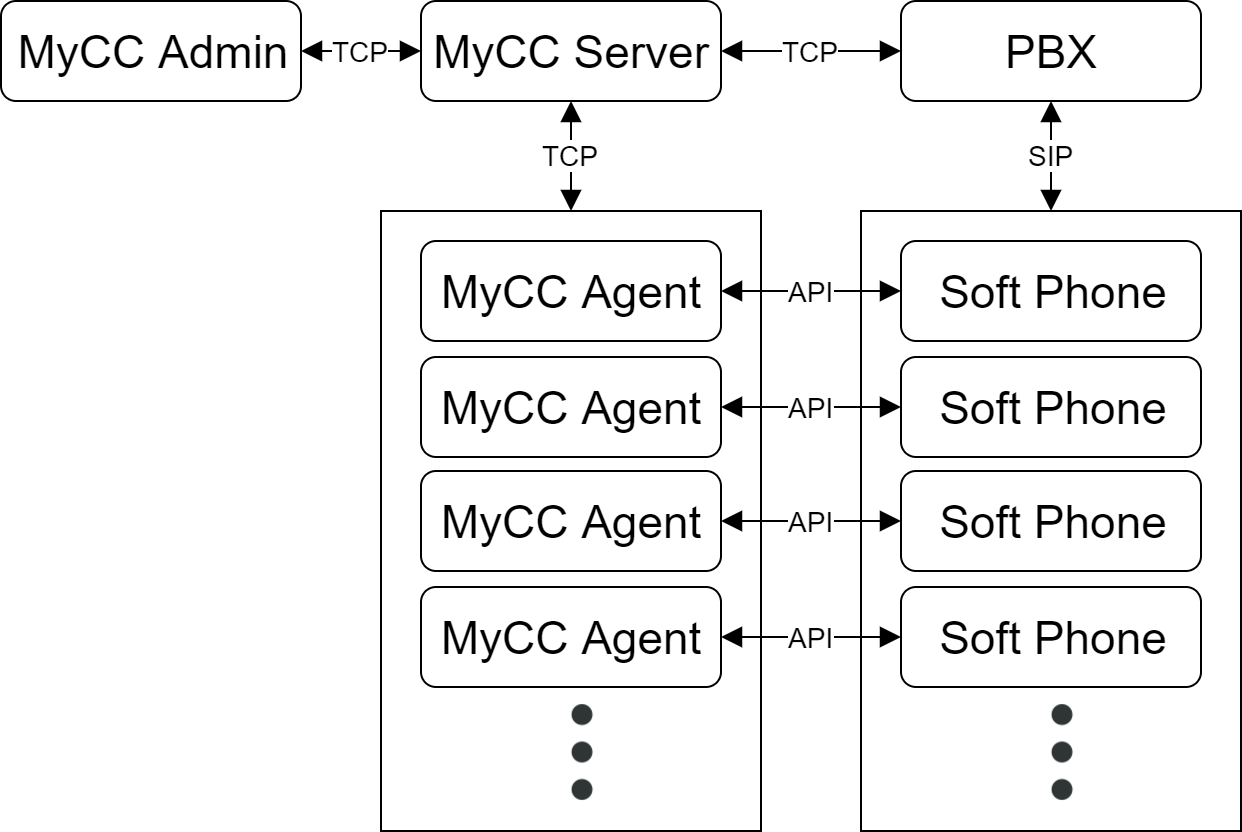
\includegraphics[scale=0.15]{img/MyCCStructure.png}
				}
    	\end{column}
    \end{columns}
\end{frame}

\begin{frame}{Einführung}{Was?}
	\center
	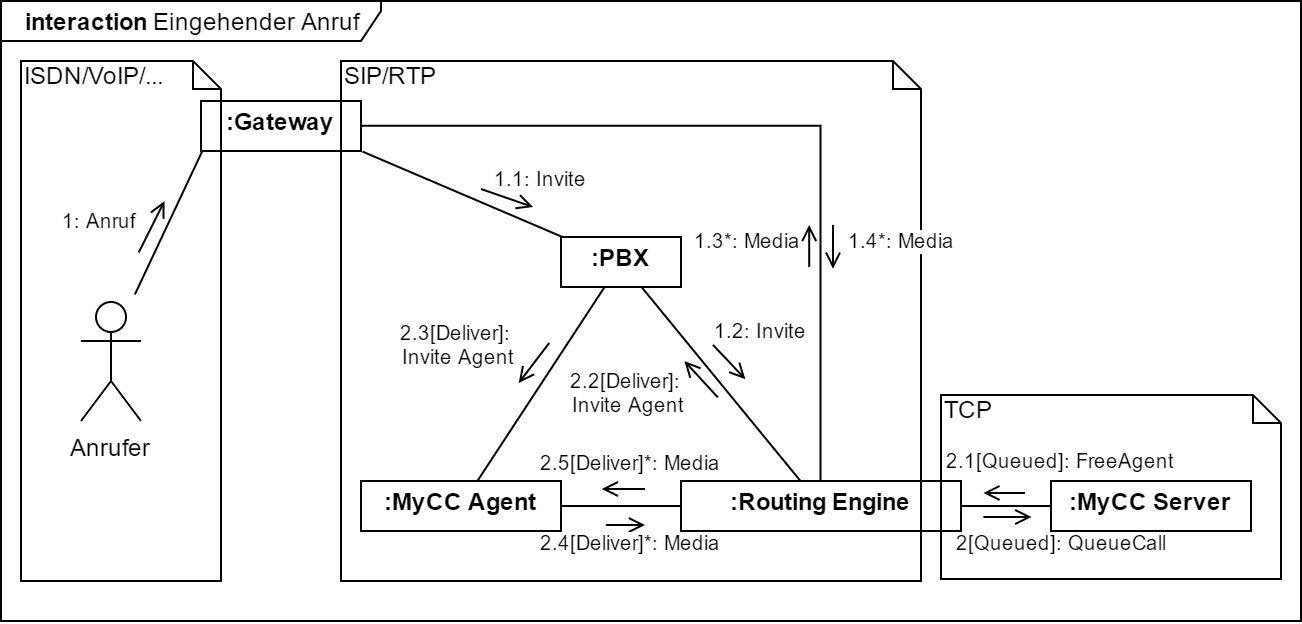
\includegraphics[width=0.9\textwidth]{img/RoutingEngineSipExplanation.png}
\end{frame}

\begin{frame}{Einführung}{Was?}
	\begin{columns}
		\begin{column}{0.5\textwidth}
			\begin{itemize}
				\item Charakteristiken domänenspezifischer Sprachen (nach \cite[S. 30ff]{Voelter:13})
				\begin{itemize}
					\item<2-> Domäne vs. General Purpose
					\item<3-> Modellieren vs. Programmieren
					\item<4-> Abstraktion vs. Maschinennähe
				\end{itemize}
			\end{itemize}
		\end{column}
		\begin{column}{0.5\textwidth}
			\only<2>
			{
				\center
				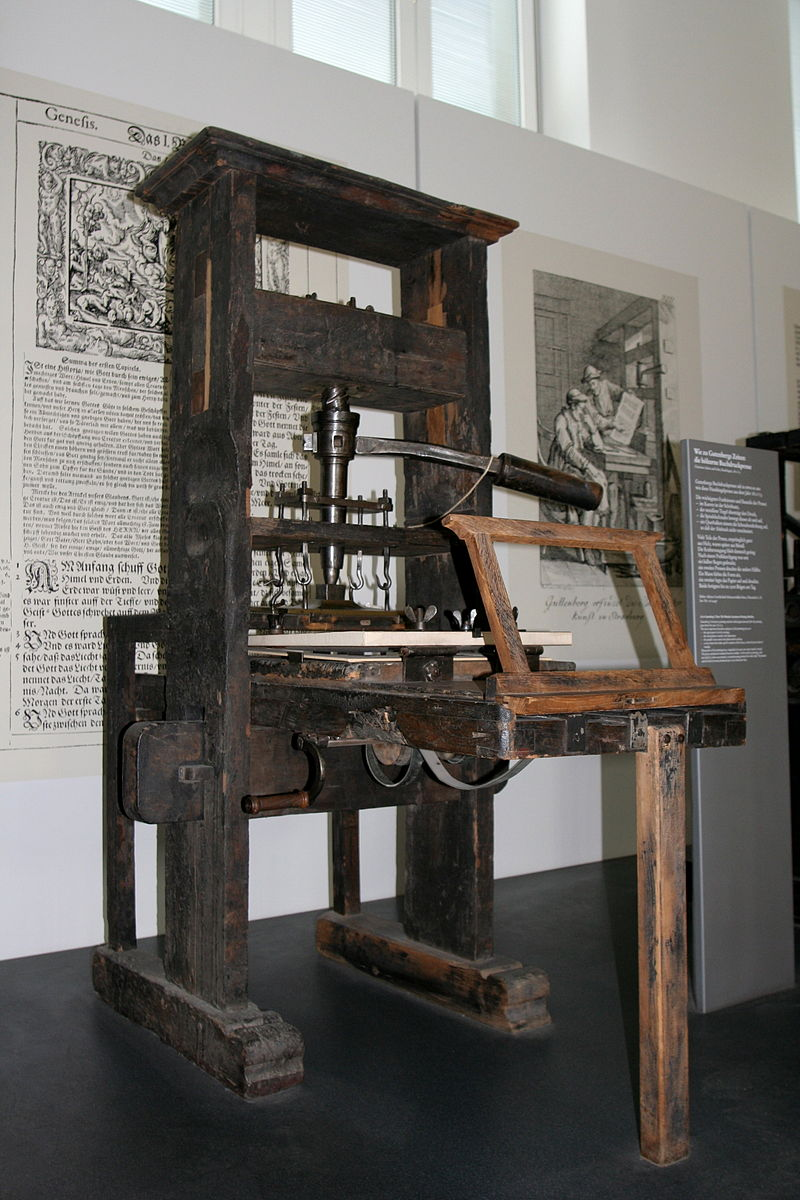
\includegraphics[width=0.4\textwidth]{img/Druckpresse.jpg}
				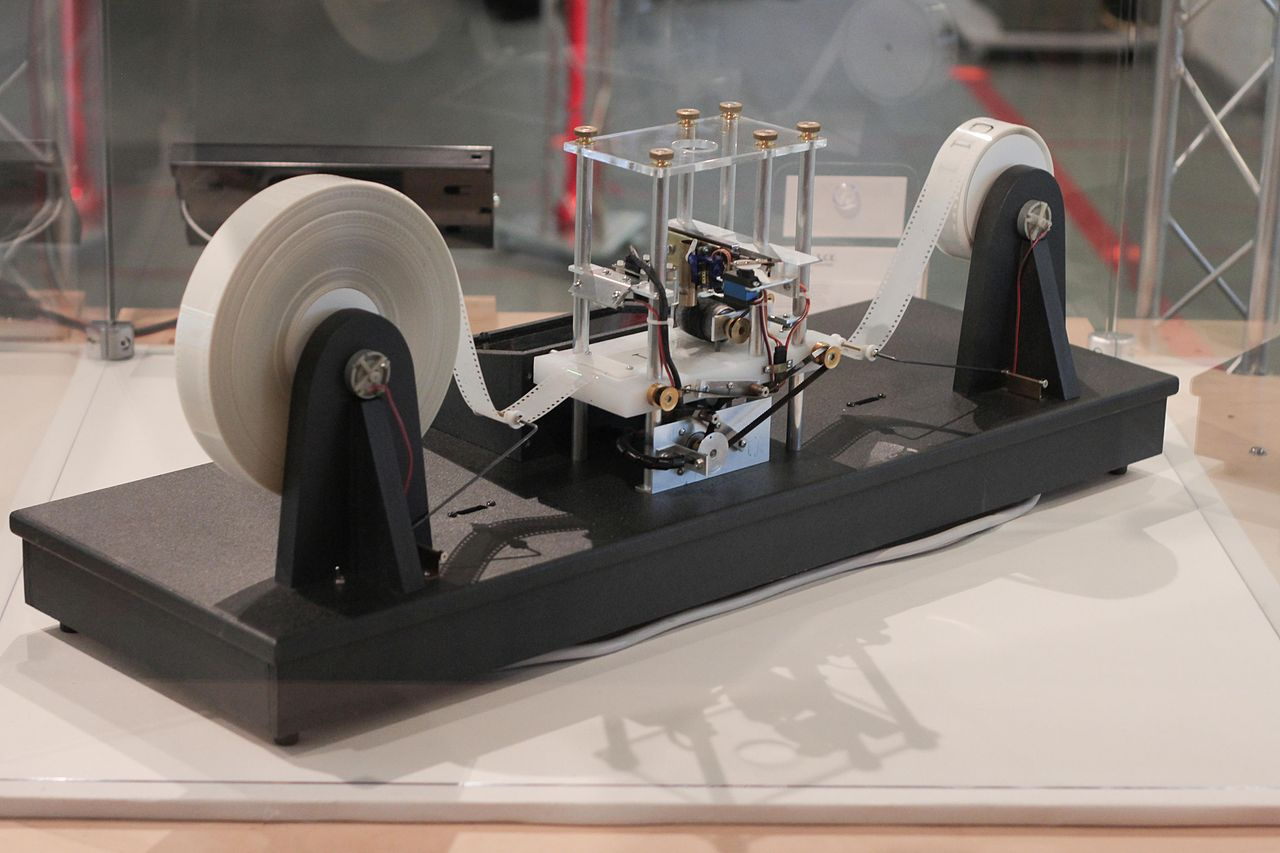
\includegraphics[width=0.58\textwidth]{img/TuringMachine.jpg}
			}
			\only<3>
			{
				\center
				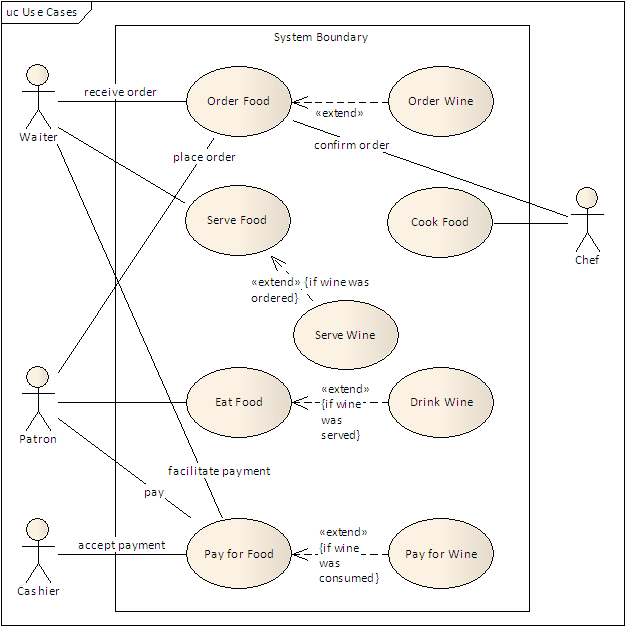
\includegraphics[width=0.49\textwidth]{img/UMLModel.png}
				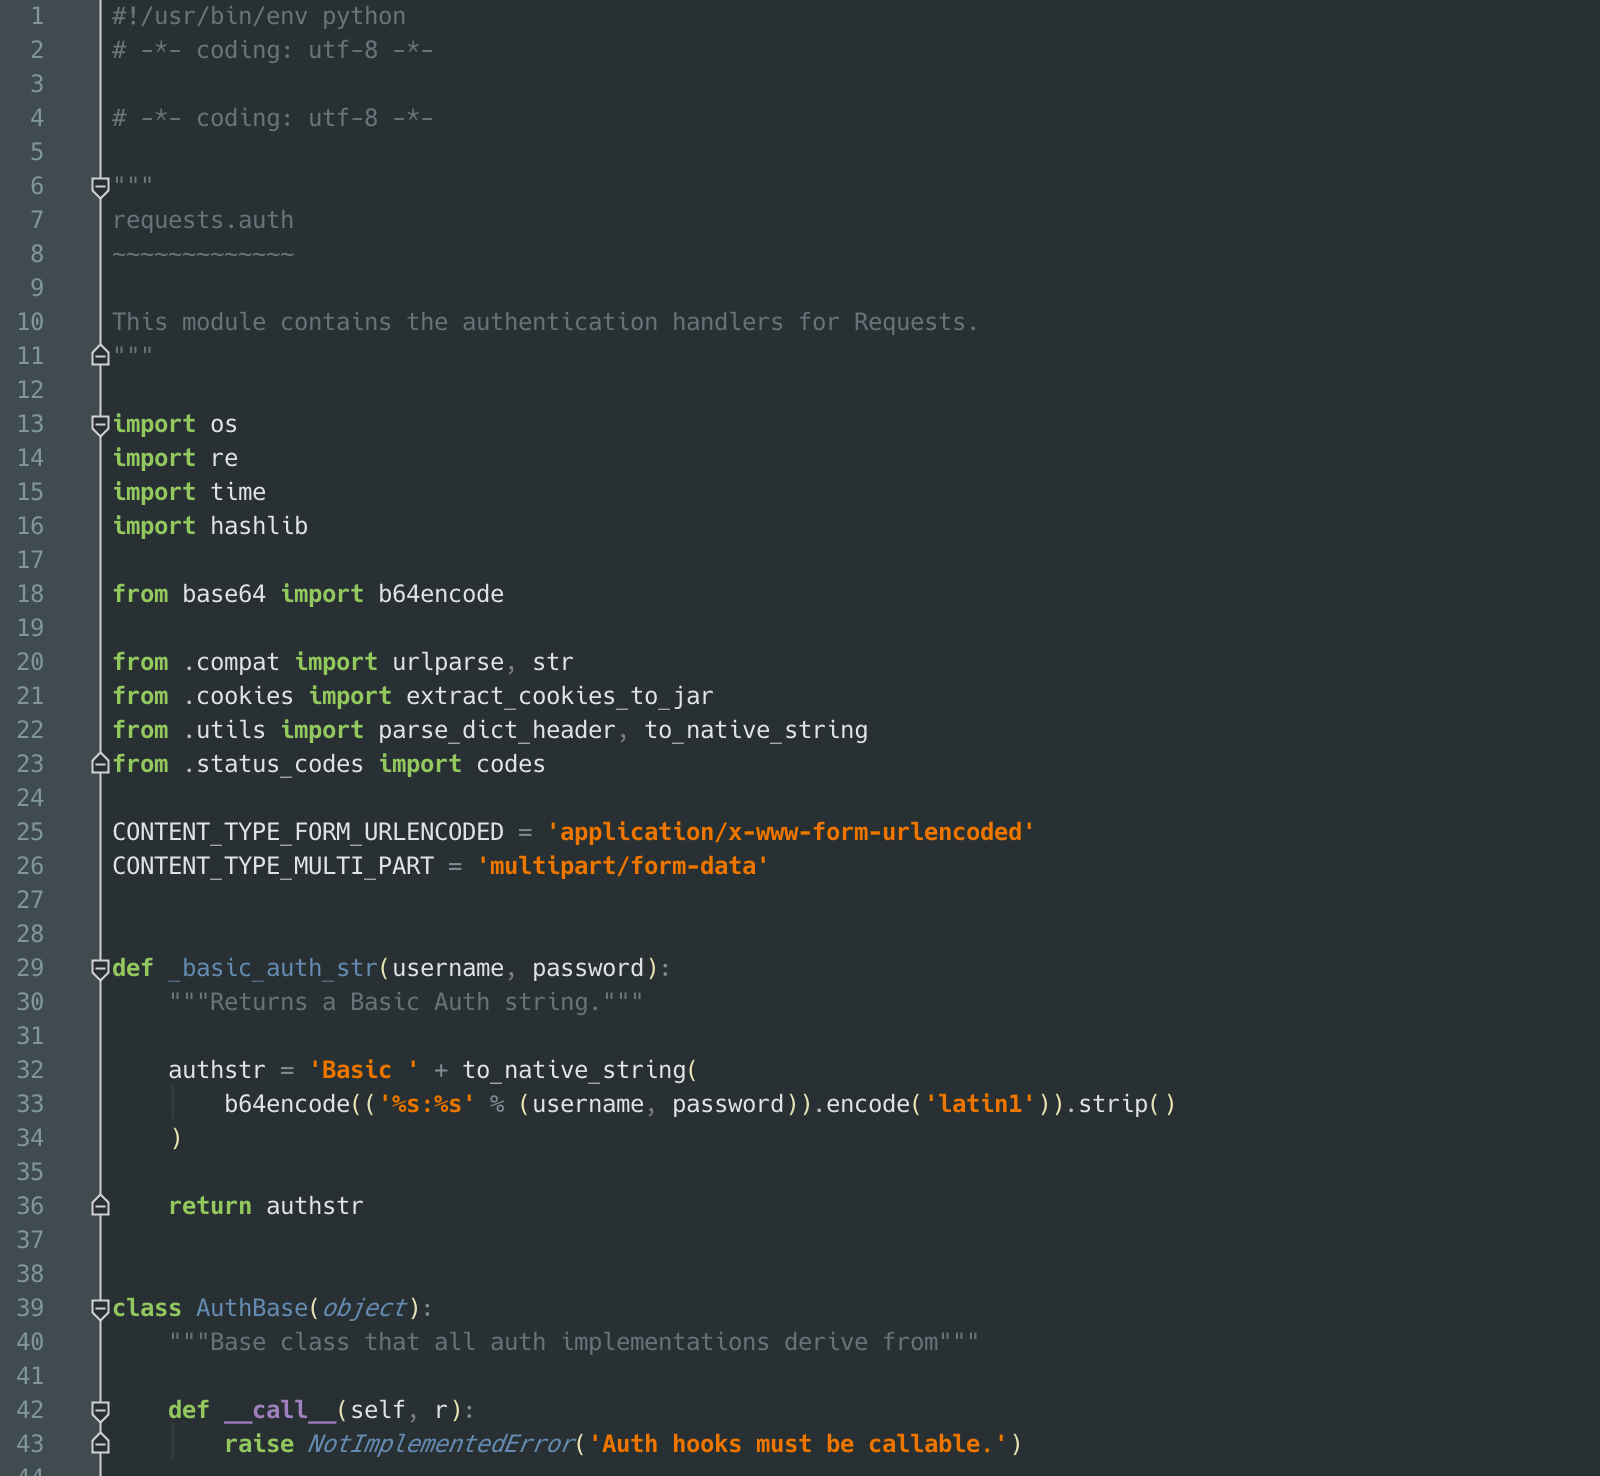
\includegraphics[width=0.49\textwidth]{img/SourceCode.png}
			}
			\only<4>
			{
				\center
				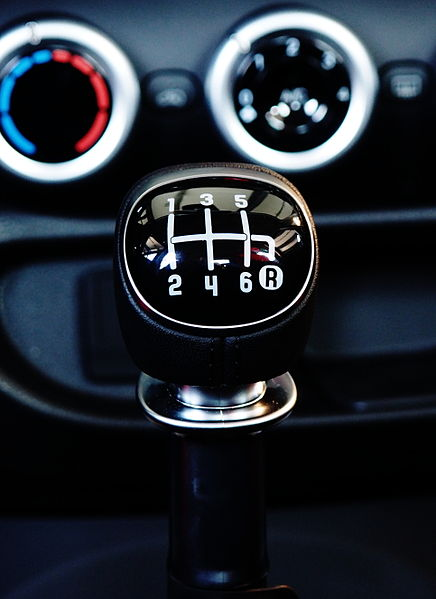
\includegraphics[width=0.33\textwidth]{img/GearShift.jpg}
				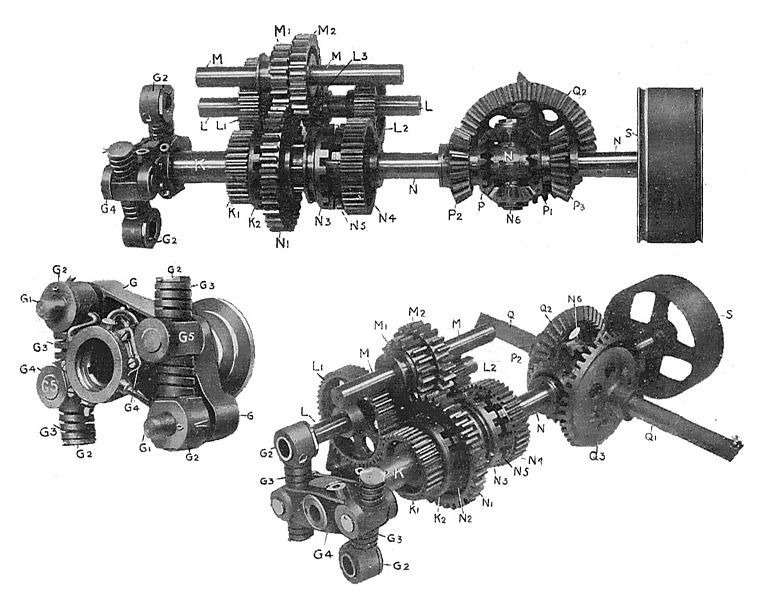
\includegraphics[width=0.64\textwidth]{img/GearShiftTechnical.jpg}
			}
		\end{column}
	\end{columns}
\end{frame}

\begin{frame}{Einführung}{Warum?}
	\begin{itemize}
		\item<1-> Kunden von MyCC wollen...
			\begin{itemize}
				\item<2-> Anpassbarkeit 
				\item<3-> Benutzerfreundlichkeit
				\item<4-> Funktionsumfang
			\end{itemize}
	\end{itemize}
\end{frame}

\begin{frame}{Entwurf}{Die Sprache}
	\only<1>
	{	
		\center
		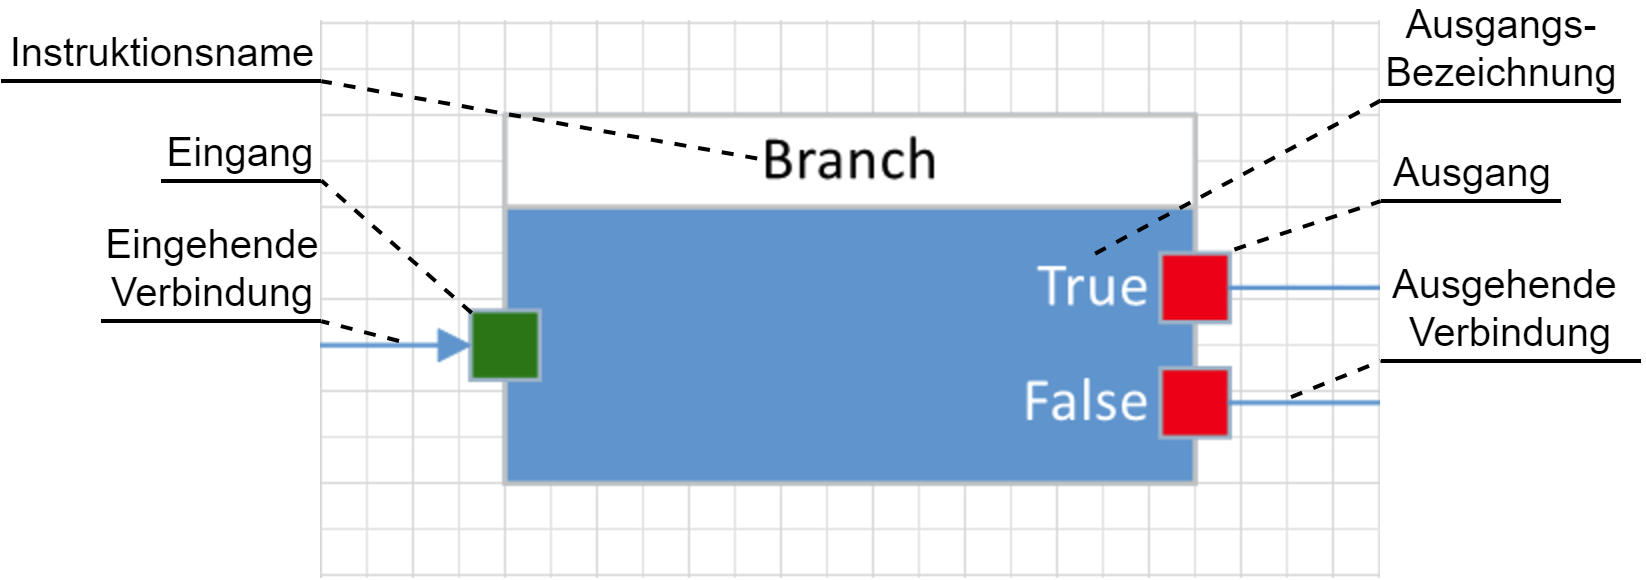
\includegraphics[width=\textwidth]{img/SingleNodeWithAnnotations.png}
	}
	\only<2>
	{
		\center
		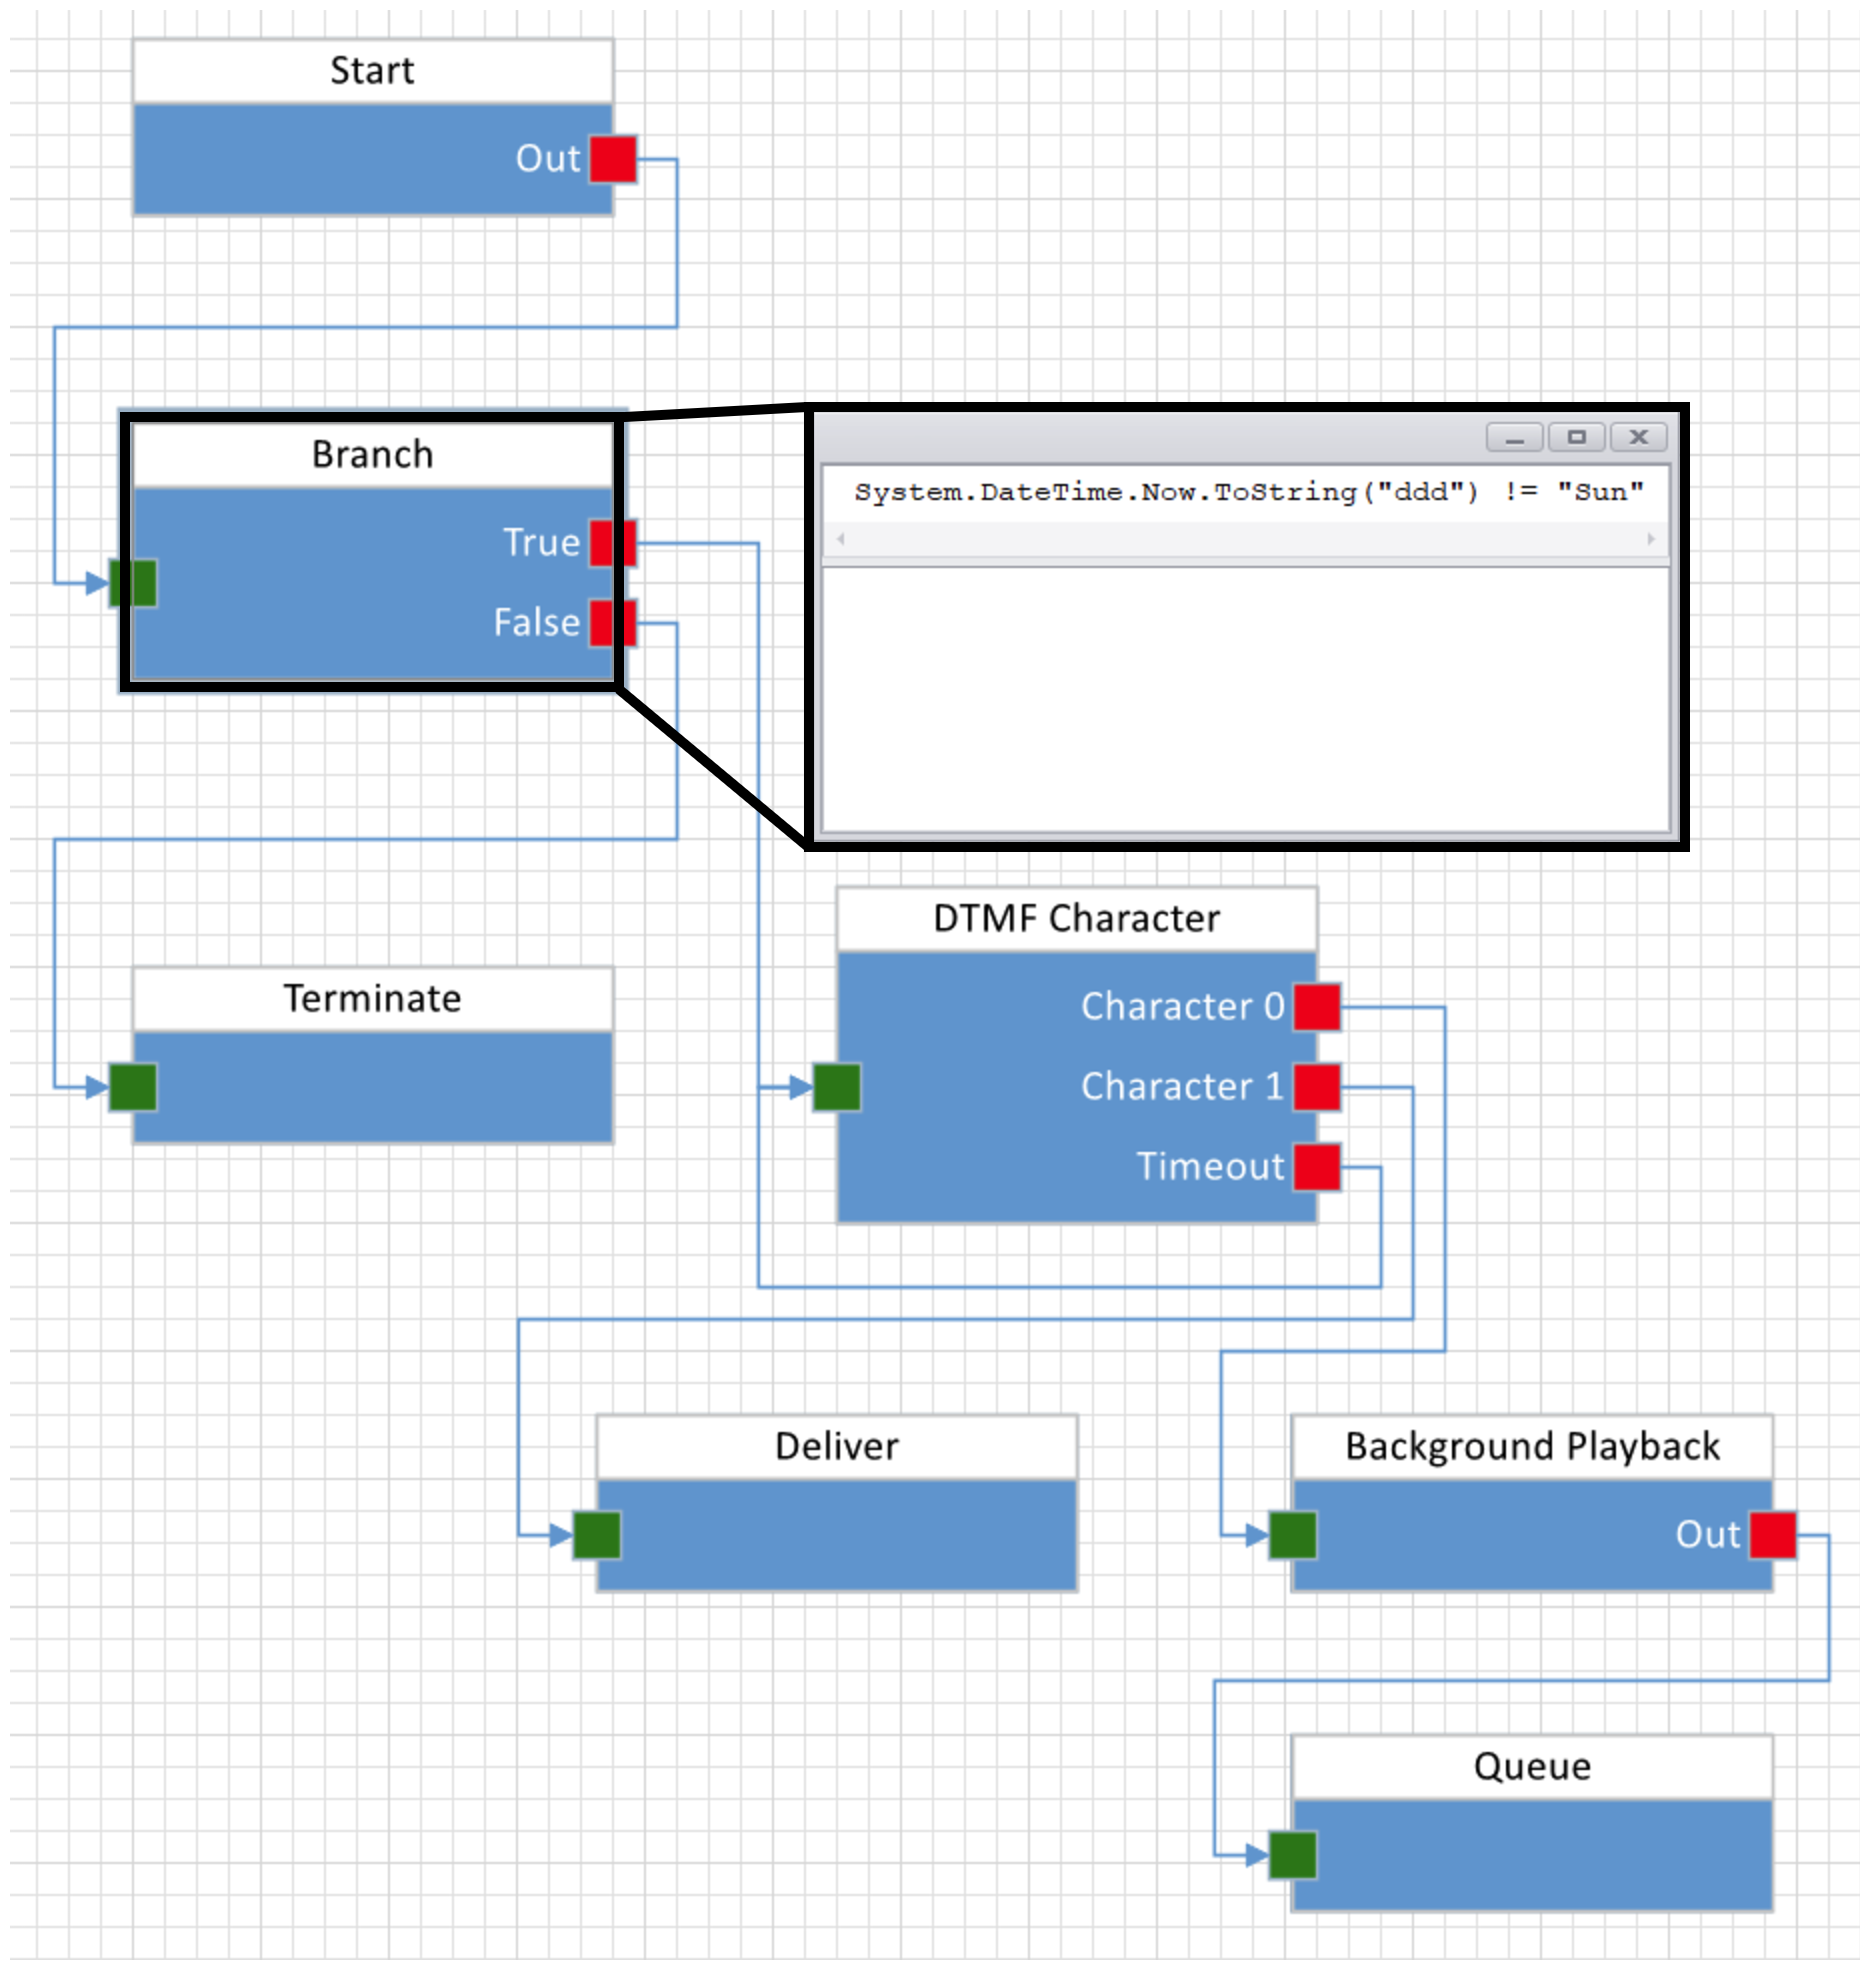
\includegraphics[scale=0.09]{img/ExampleFlowCodeHighlighted.png}
	}
	\only<3>
	{
		\center
		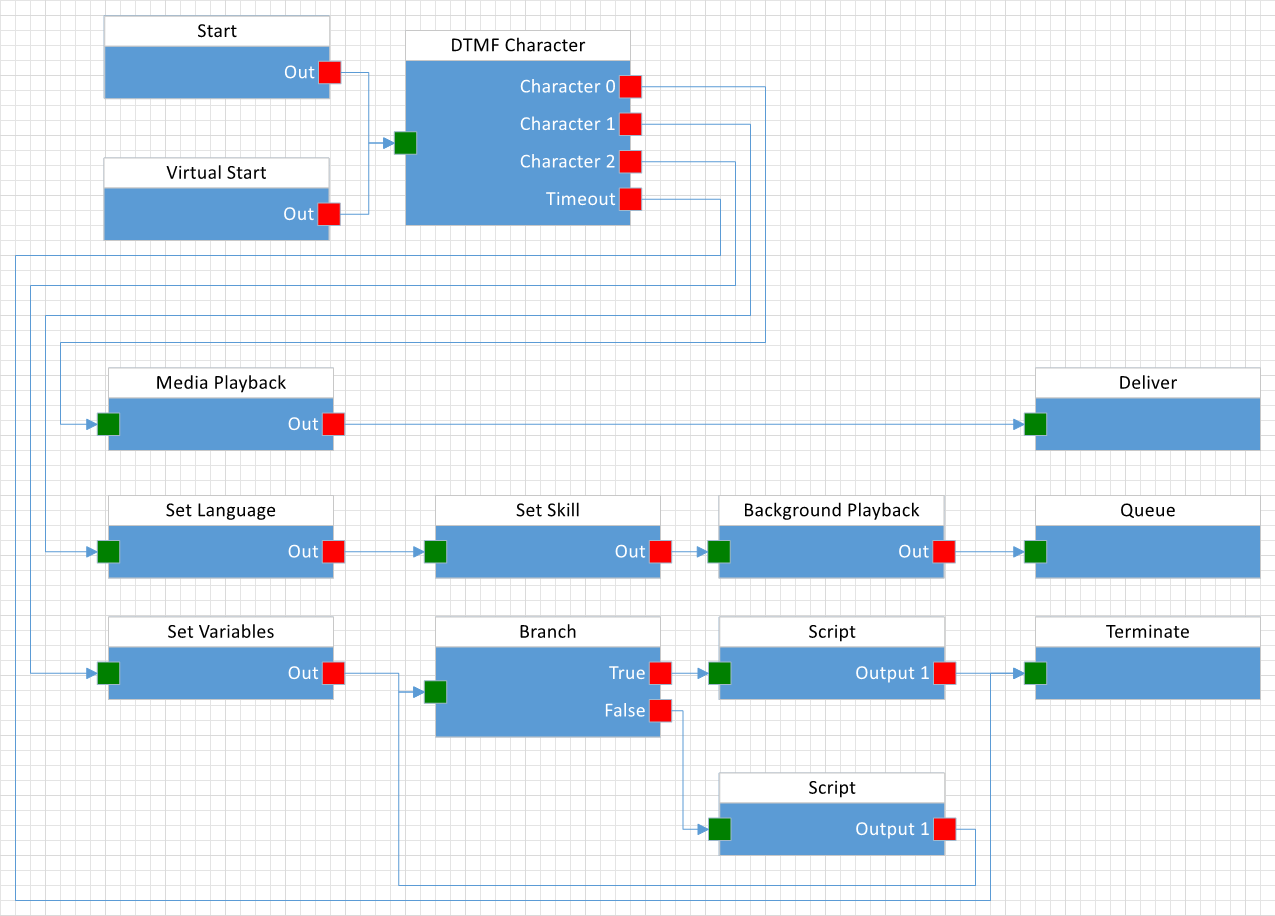
\includegraphics[width=0.6\textwidth]{img/TestRouting.png}
	}
	\only<4>
	{
		\center
		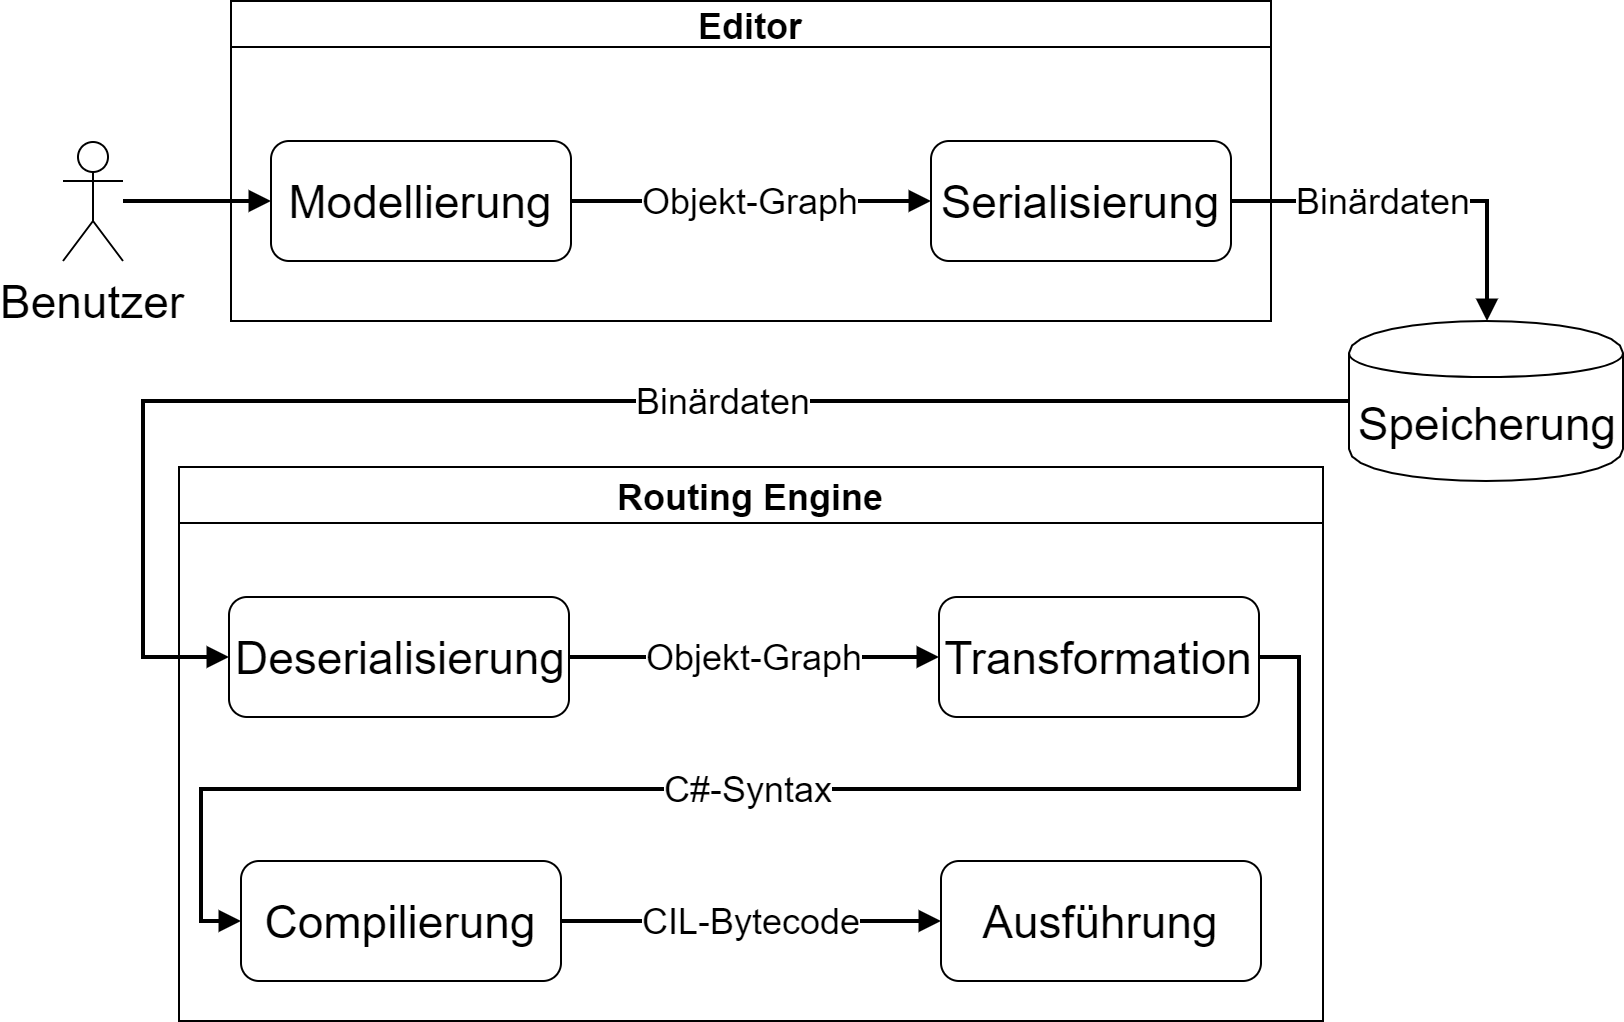
\includegraphics[width=0.7\textwidth]{img/Verarbeitungsschritte.png}
	}
\end{frame}

\begin{frame}{Implementierung}{Editor}
	\only<1>
	{	
		\center
		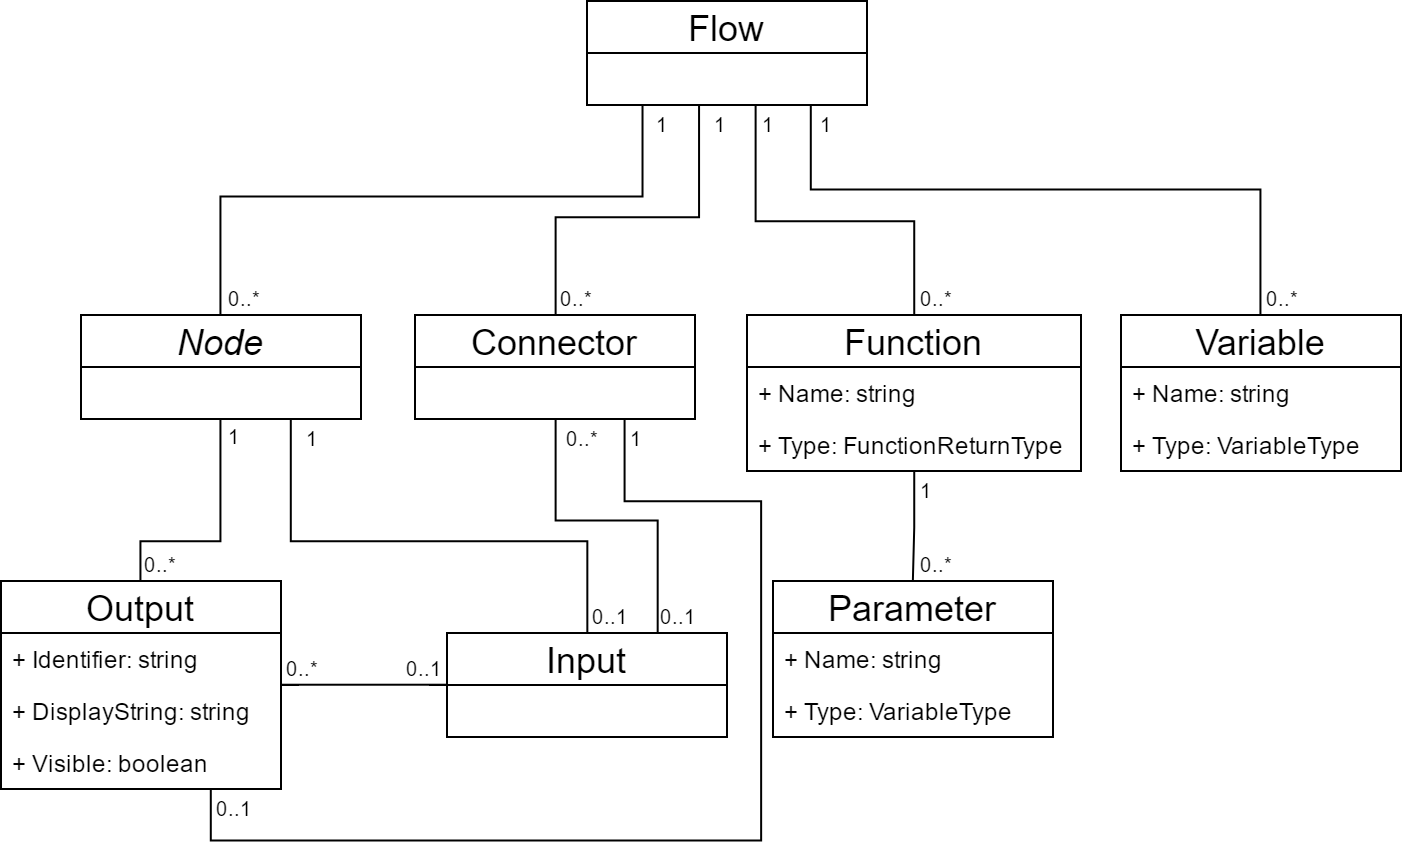
\includegraphics[width=0.7\textwidth]{img/FlowClassStructure.png}
	}
	\only<2>
	{
		\center
		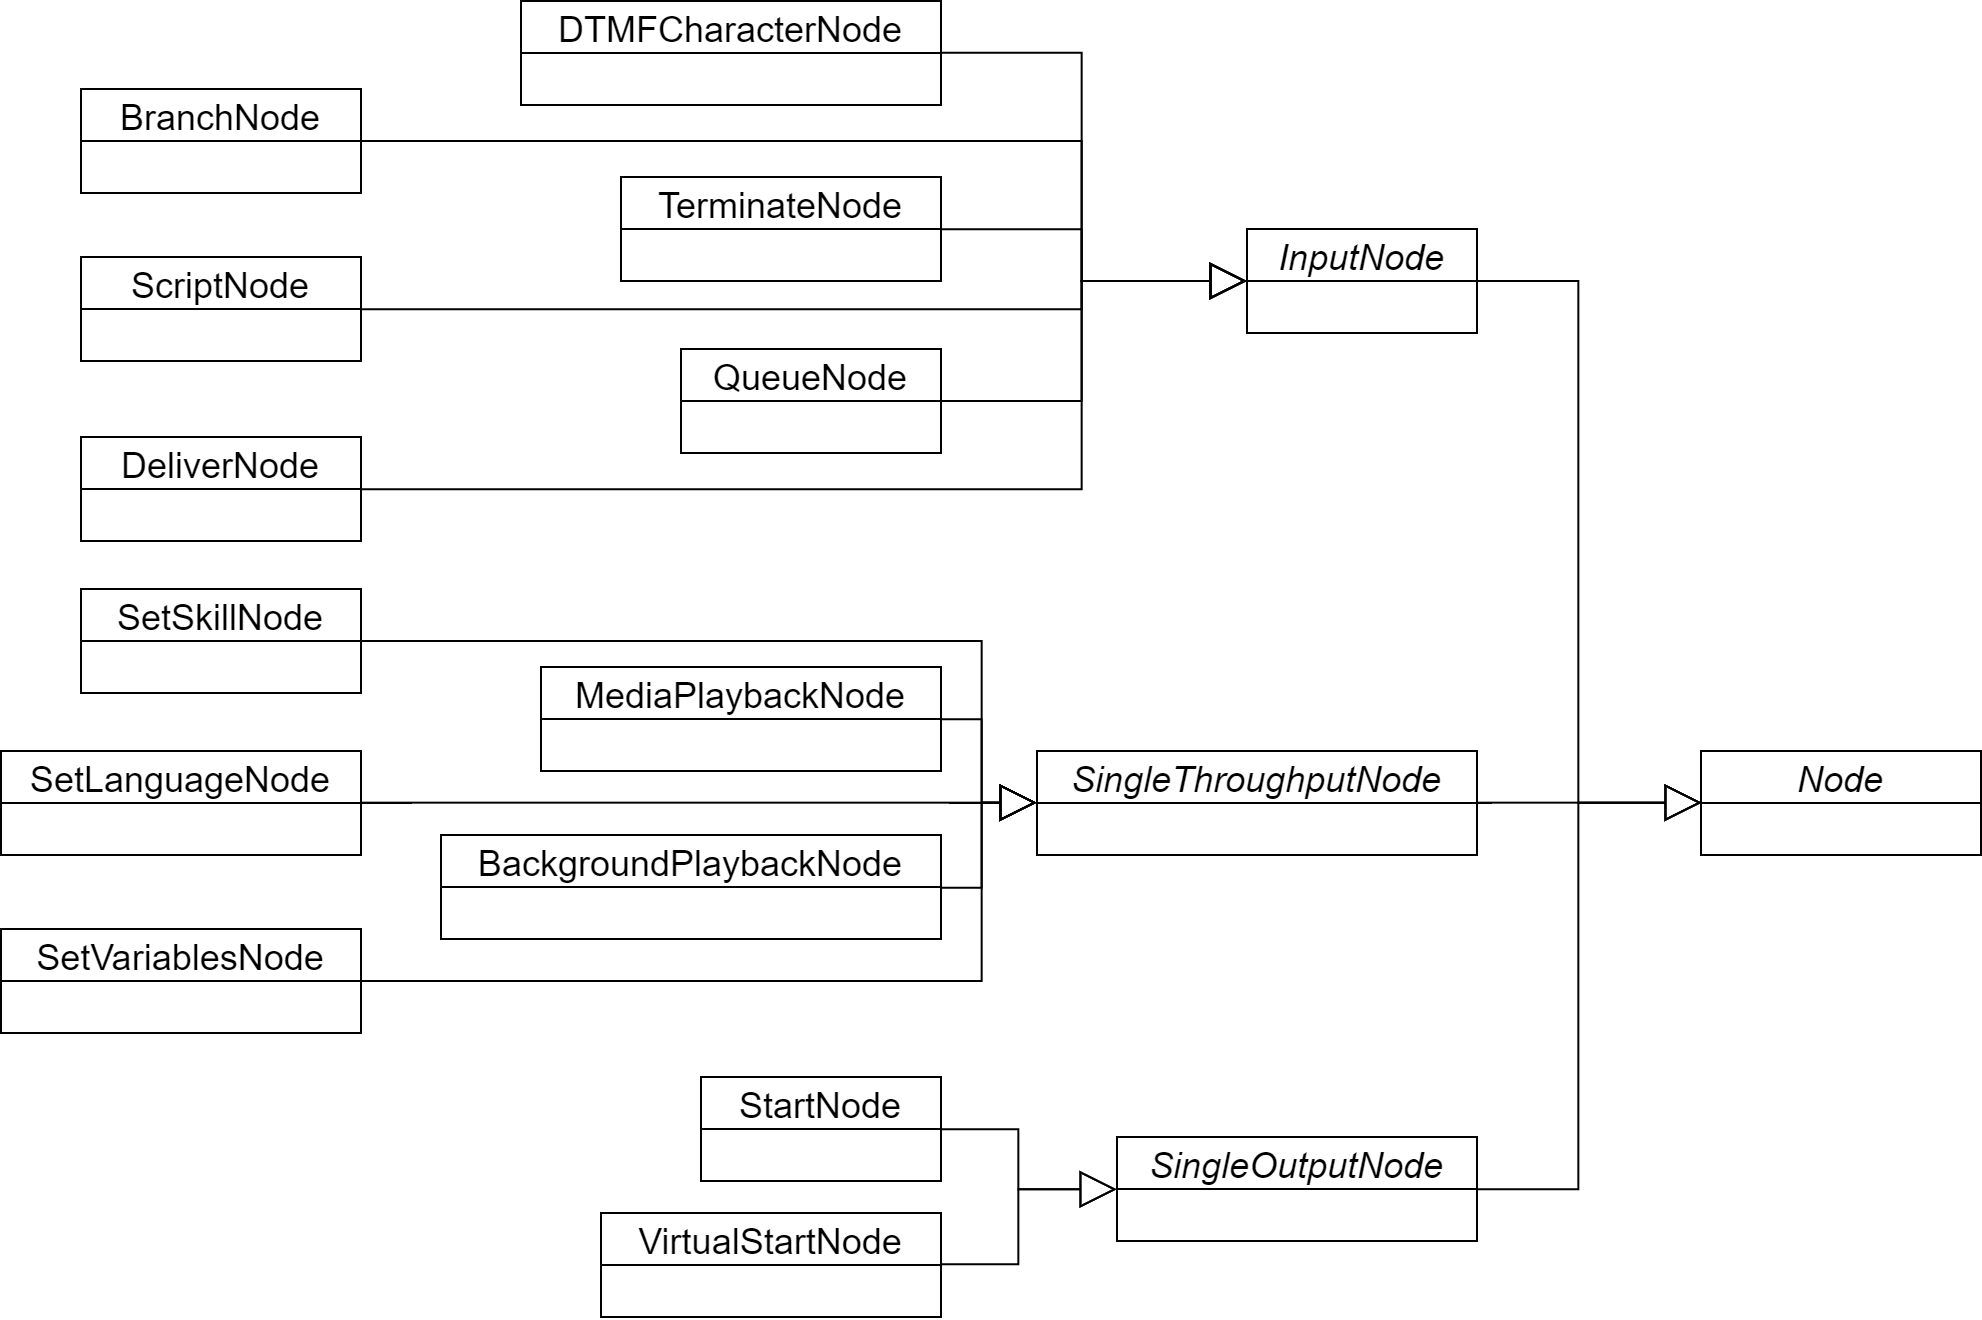
\includegraphics[width=0.65\textwidth]{img/NodeHierarchy.png}
	}
\end{frame}

\begin{frame}[fragile]{Implementierung}{Transformation}
	\begin{columns}[T]
		\begin{column}{0.4\textwidth}
			\center
			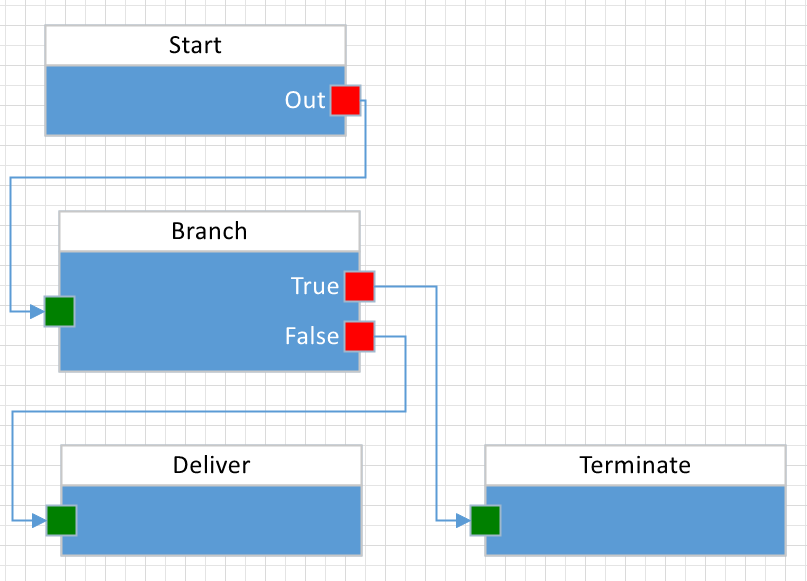
\includegraphics[width=\textwidth]{img/FlowToCodeExample.png}
		\end{column}
		\begin{column}{0.6\textwidth}
			\only<2>
			{
				\lstinputlisting[language=custom, firstline=1, lastline=8]{Code/FlowToCode.cs}
			}
			\only<3>
			{
				\lstinputlisting[language=custom, firstline=8, lastline=28]{Code/FlowToCode.cs}
			}
			\only<4>
			{
				\lstinputlisting[language=custom, firstline=30, lastline=38]{Code/FlowToCode.cs}
			}
			\only<5>
			{
				\lstinputlisting[language=custom, firstline=39, lastline=63]{Code/FlowToCode.cs}
			}
		\end{column}
	\end{columns}
\end{frame}

\section*{Schluss}
\begin{frame}
	\begin{center}
		\huge{Vielen Dank für die Aufmerksamkeit}
	\end{center}
	\begin{center}
		\Huge{Fragen?}
	\end{center}
\end{frame}

\begin{frame}[allowframebreaks]{\bibname}
\bibliography{literatur}     %BibTeX-Datei literatur.bib
\end{frame}


\end{document}
